

\documentclass{beamer}

\mode<presentation> {


\usetheme{Madrid}



\setbeamertemplate{footline}[page number] 

\setbeamertemplate{navigation symbols}{} % To remove the navigation symbols from the bottom of all slides uncomment this line
}

\usepackage{graphicx} 


\usepackage{comment}
\usepackage{tikz}
\usepackage{booktabs} 
\usepackage{tikz-cd}
\usepackage{fontawesome}
\usepackage{apacite}
\renewcommand\bibliographytypesize{\footnotesize}
\usepackage{mathtools}
%\usepackage {tikz}
\usepackage{tkz-graph}
\GraphInit[vstyle = Shade]
\tikzset{
  LabelStyle/.style = { rectangle, rounded corners, draw,
                        minimum width = 2em, fill = yellow!50,
                        text = red, font = \bfseries },
  VertexStyle/.append style = { inner sep=5pt,
                                font = \normalsize\bfseries},
  EdgeStyle/.append style = {->, bend left} }
\usetikzlibrary {positioning}
%\usepackage {xcolor}
\definecolor {processblue}{cmyk}{0.96,0,0,0}


\title[Short title]{Progress Report} 

\author{Shakil Rafi} 
\institute[University of Arkansas] 
{
University of Arkansas \\ 
\medskip
}
\date{\today} 

\begin{document}
\nocite{*}
\begin{frame}
\titlepage 
\end{frame}

\begin{frame}
\frametitle{Table of Contents} 
    \tableofcontents 
\end{frame}
\begin{frame}{What to Solve}
    We seek to solve dynamic equilibrium equations. The formulation from Liu and Quek assumes among other things:
    \begin{enumerate}
        \item \textit{Linear Elastic} Deformation grows proportionally with external force.
        \item \textit{Isotropic} Material property is direction independent.
    \end{enumerate}
    We distinguish between four kinds of objects: beams, trusses, plates and shells.
\end{frame}
\begin{frame}{What to Solve}
    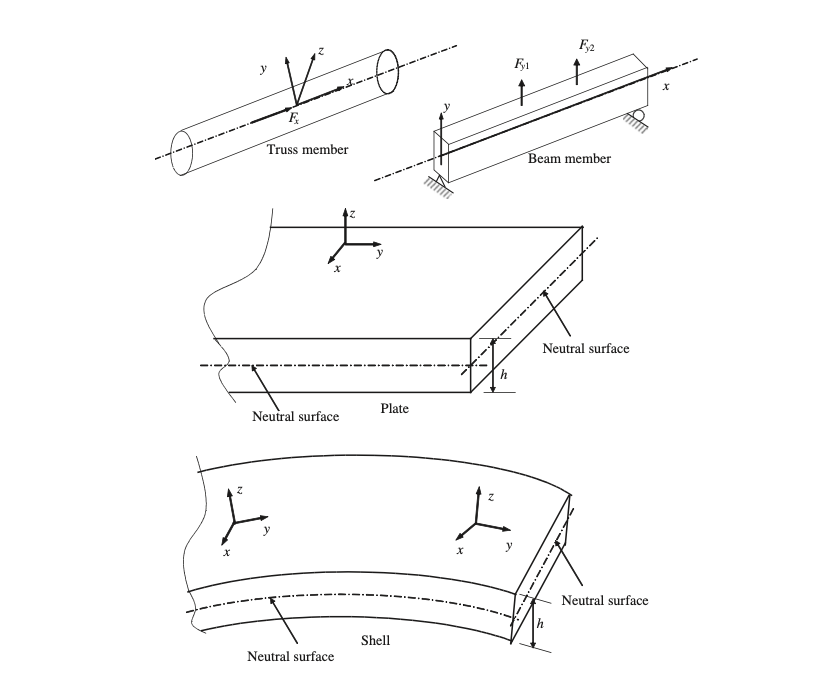
\includegraphics[scale = 0.35]{TypesOfObjects.png}
\end{frame}
\begin{frame}{What to Solve}
    Taking a queue from Liu and Quek, we start off by defining DEE for an idealized infinitesimal, linearly elastic, isotropic material.
    \quad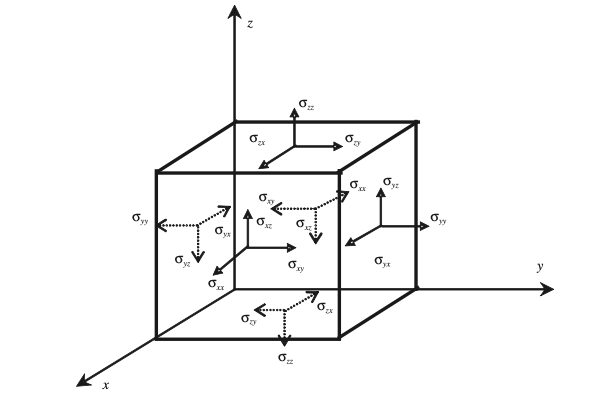
\includegraphics[scale = 0.4]{Cube.png}

    Observe that because of equilibrium $\sigma_{xy} = \sigma_{yx}; \sigma_{xz} = \sigma_{zx}; \sigma_{yz}= \sigma_{yz}$ 
    Which give sus the stress tensors: $\sigma^T = \{\sigma_{xx},\sigma_{yy},\sigma_{zz},\sigma_{yz},\sigma{xz},\sigma{xy}\}$
\end{frame}
\begin{frame}{What to Solve}
    
\end{frame}

\end{document}


